%%%%%%%%%%%%%%%%%%%%%%%%%%%%%%%%%%%%%%%%%%%%%%%%%%%%%%%%%%%%%%%%%%%%%%%%%%%
%% This file is part of the book
%%
%% Algorithmic Graph Theory
%% http://code.google.com/p/graph-theory-algorithms-book/
%%
%% Copyright (C) 2009, 2010 Minh Van Nguyen <nguyenminh2@gmail.com>
%%
%% See the file COPYING for copying conditions.
%%%%%%%%%%%%%%%%%%%%%%%%%%%%%%%%%%%%%%%%%%%%%%%%%%%%%%%%%%%%%%%%%%%%%%%%%%%

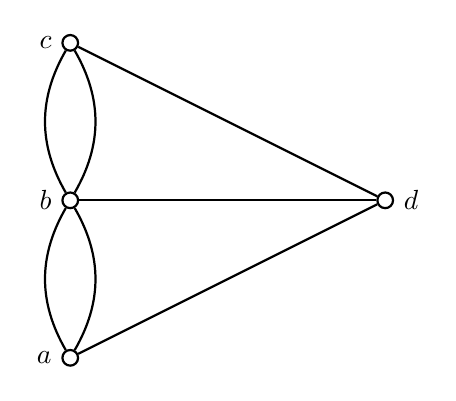
\begin{tikzpicture}
[nodedecorate/.style={shape=circle,inner sep=2pt,draw,thick},%
  linedecorate/.style={-,thick}]
%% nodes or vertices
\foreach \nodename/\x/\y/\direction/\navigate in {
  a/0/0/left/west, b/0/2/left/west, c/0/4/left/west, d/4/2/right/east}
{
  \node (\nodename) at (\x,\y) [nodedecorate] {};
  \node [\direction] at (\nodename.\navigate) {$\nodename$};
}
%% edges or lines
\path
\foreach \startnode/\endnode in {a/d, b/d, c/d} {
  (\startnode) edge[linedecorate] node {} (\endnode)
};
\path
\foreach \startnode/\endnode in {a/b, b/c} {
  (\startnode) edge[linedecorate,bend left] node {} (\endnode)
};
\path
\foreach \startnode/\endnode in {c/b, b/a} {
  (\startnode) edge[linedecorate,bend left] node {} (\endnode)
};
\end{tikzpicture}
